\documentclass{article}
\usepackage[T1]{fontenc}
\usepackage{lmodern}
\usepackage{graphicx}
\usepackage{amsmath,amssymb}
\usepackage[a4paper,margin=2cm]{geometry}
\usepackage[absolute,overlay]{textpos}
\setlength{\TPHorizModule}{1mm}
\setlength{\TPVertModule}{1mm}
\usepackage[indonesian]{babel}
\usepackage{hyperref}
\setlength{\emergencystretch}{2em}
% unit: Halaman 31

\begin{document}

% === Halaman 31 (llm) ===

Sumber: William Stalling, Cryptography and Network Security\nOverview & Chapter 1

\vspace{60mm}

\begin{center}
\textbf{Passive Attack : Interception}
\end{center}

% deskripsi: Diagram ilustrasi serangan pasif berupa intersep pesan antara Bob dan Alice melalui Internet, di mana pihak ketiga bernama Darth menyadap konten pesan.
% bbox normalisasi: [0.1500, 0.1900, 0.7900, 0.7700]
\begin{textblock*}{134.40mm}(31.50mm,56.43mm)
\noindent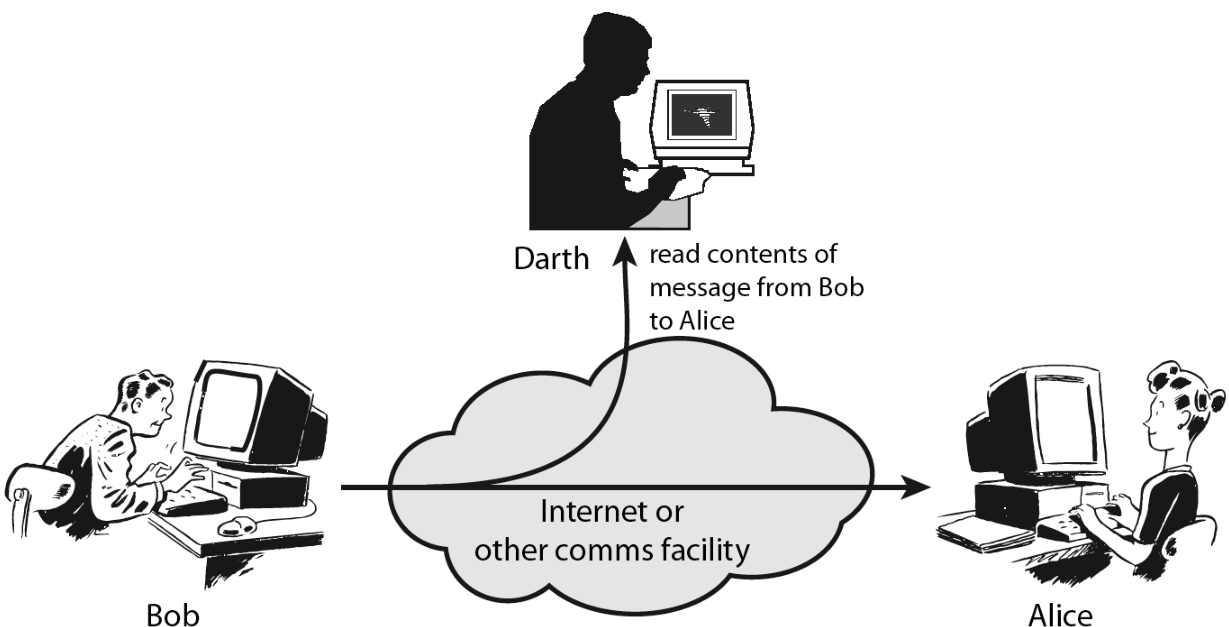
\includegraphics[width=134.40mm,height=172.26mm]{../../images/llm/page_031_img_01.png}%
\end{textblock*}

\end{document}
